\section{Experimental Design}\label{sec:evaluation}
The evaluation targets four questions: whether specialization improves professional task quality; whether retained updates improve unseen work; whether any gains justify total resources and human effort; and whether improvement preserves previously useful capabilities. This manuscript contains the method and experimental design; performance measurements are not yet reported.

\paragraph{Task families and partitions.}
The primary family is evidence-based analytical reporting: each task provides a fixed source bundle, a computational question, and a deliverable contract. Acceptance requires reproducible calculations, support for load-bearing claims, and agreement between the rendered report and canonical results. A second family uses software maintenance tasks with executable functional checks and exact repository snapshots. Enrollment requires at least three dependent stages, an intermediate artifact consumed and checked in a later stage, and an independently checkable final deliverable. These requirements apply to the task contract, not the number of agents. We record required stages, tool interactions, and input resource size. The reuse horizon $T$ counts subsequent assignments to the retained organization; it does not assert a particular single-task duration or context length.

Tasks are partitioned by source provenance or repository, before development, into update tasks, unseen future tasks from the same family, and a retained-capability test set. Reworded questions over the same evidence and related issues from one repository remain in the same partition. A separate, untouched family tests cross-domain transfer only when its tools and contracts are already compatible with the starting package; results from this setting are reported separately from within-domain generalization. Figure~\ref{fig:evolution} specifies the information boundary.

\begin{figure}[!t]
\centering
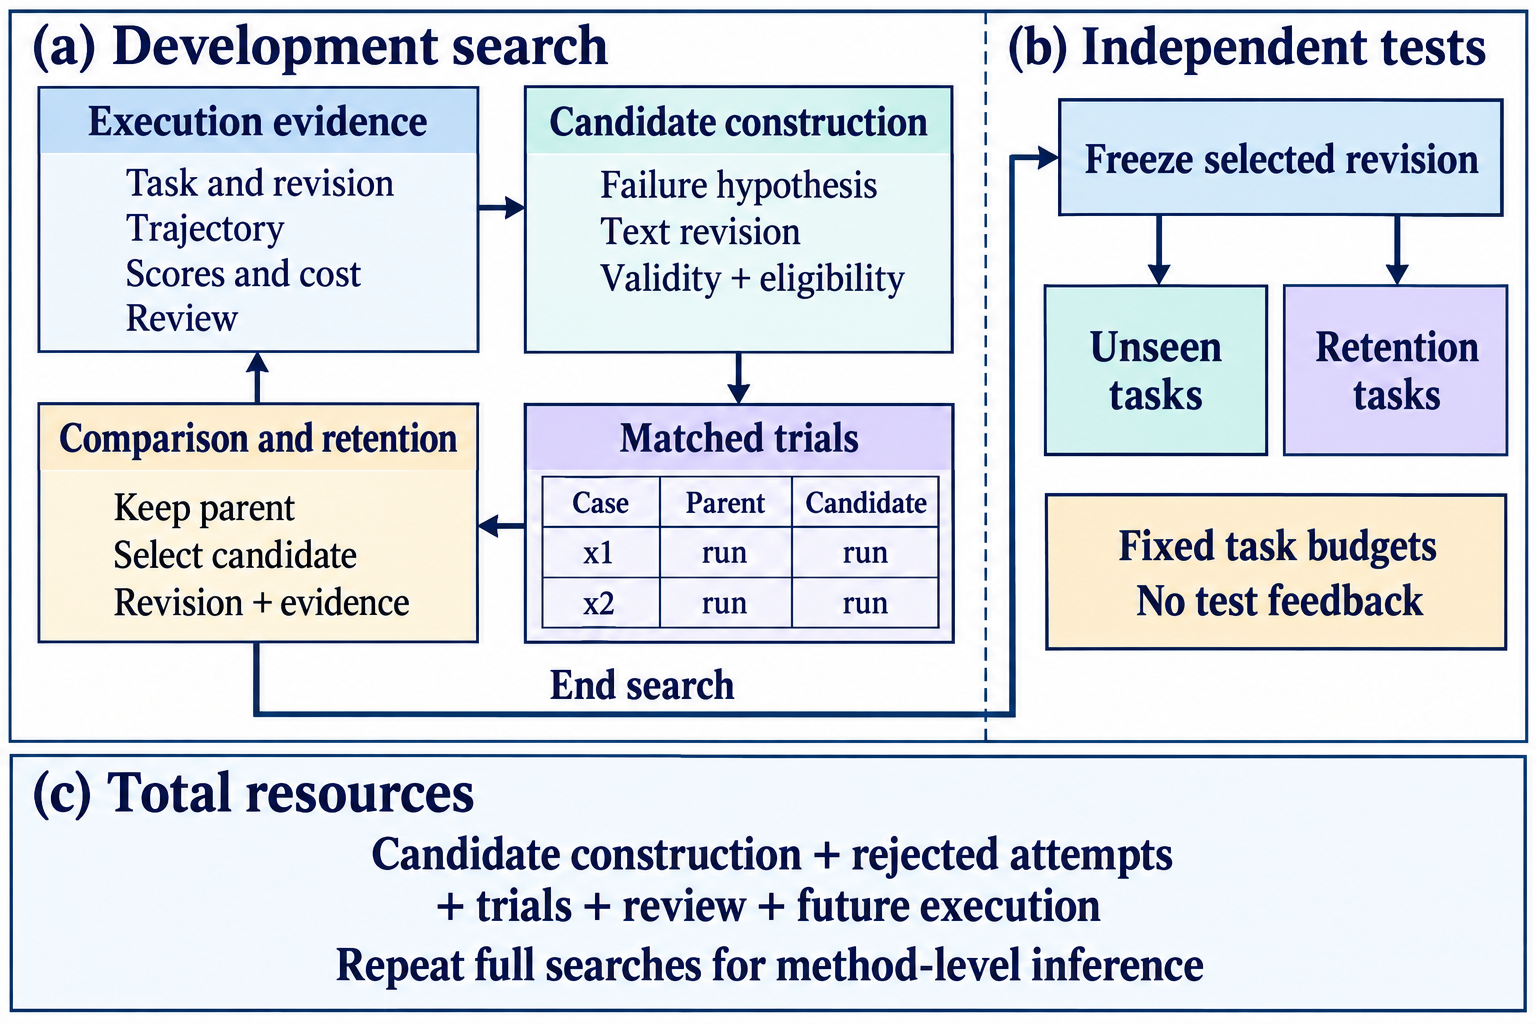
\includegraphics[width=\linewidth]{figures/evolution.png}
\caption{Organizational development and independent evaluation. Development trials supply evidence for candidate construction and retention. The final selected organization is frozen before independent unseen-task and prior-capability evaluation. The pairing matrix denotes trial slots, not measured results. Total resource accounting includes failed search attempts. A new search episode uses fresh partitions; test outcomes do not return to the same search.}
\label{fig:evolution}
\end{figure}


\paragraph{Controlled comparisons.}
All arms use the same foundation model, inference configuration, domain input access, and total resource ceiling. Table~\ref{tab:arms} defines successive organizational changes. For the collaboration contrast, one frozen generic instruction set supplies both the single agent and the fixed team with identical planning, execution, and checking procedures. The single agent receives the complete set, can use the union of the team's tools, and performs the same responsibilities within one iterative context. The team distributes those procedures to their corresponding roles; only participant addressing and the messages needed for delegation change. This contrast estimates the effect of distributing the same procedural knowledge across communicating agents, including its context and coordination costs. Neither arm is restricted to a one-shot response.

The fixed generic and specialized teams share the same role roster, workflow declarations, and capability allocations. Specialization changes the domain procedures, reference bindings, and output-contract instructions. The task's acceptance rubric and underlying source access remain identical. Each family's concrete instruction sets and deployment mappings are frozen before development, so a stronger manually authored baseline cannot be introduced after seeing test outcomes.

\begin{table}[!htb]
\centering\small
\begin{tabularx}{\linewidth}{@{}lYYY@{}}
\toprule
Arm & Organization & Domain procedures & Retained updates \\
\midrule
Single agent & One iterative tool-using agent & Complete generic instruction set & None \\
Fixed team & Generic expert roles & Same generic set, assigned by role & None \\
Specialized team & Fixed domain organization & Explicit procedures and contracts & None \\
EEO--text & Same initial specialized team & Same initial package & Experience-driven text revision \\
\bottomrule
\end{tabularx}
\caption{Primary comparisons. EEO--text follows the released text-authoring policy, with an additional research eligibility check on each realized diff. Structural search requires a separate generator and study arm.}
\label{tab:arms}
\end{table}

Search costs are charged before future execution. Each arm receives the same episode-wide ceiling $B$ over the same number of assigned future tasks. Before inspecting any test outcome, each arm allocates its post-search remainder to fixed per-task caps whose sum does not exceed that remainder. An arm with no search can allocate larger inference caps. Caps are not recycled across test tasks, and each execution starts from its prescribed isolated workspace. This prevents a costly early task from reducing a later task's allowance. Unfinished assigned tasks remain in the quality denominator. A supplementary comparison fixes per-task inference cost to expose the mechanism's effect without amortization; it is labeled separately and reports search overhead.

\paragraph{Optimizer control.}
The protocol compares EEO--text with a GEPA-based adaptation on the same initial package, eligible text surface, feedback access, model, and total budget \citep{gepa}. GEPA's execution modules are LLM components with inputs, outputs, and trajectories; package files are their editable parameters, not execution modules. An orchestrator or expert can consume several files, and a shared skill can influence several experts.

Before execution, the adapter must freeze a mapping from every eligible file and descriptive manifest field to its consuming modules and visible execution evidence. It must specify the feedback attached to shared resources, the update policy for a resource used by multiple modules, and how a parameter update reconstructs one complete candidate package. Shared content has one canonical value; it is not independently rewritten into conflicting role-specific copies. Both optimizers start from the same development inputs and pre-existing evidence, with identical feedback interfaces and visible fields. Each receives and pays for the observations generated by its own candidate trials; the methods do not exchange search trajectories. Integrity checks and held-out tests are identical.

The adaptation preserves GEPA's candidate pool and ancestry, Pareto-based candidate sampling, declared module-selection policy, and minibatch evaluation before broader development-set scoring. The reference version, reflection prompt, sampling sizes, selection policy, optional merge setting, and stopping rule are recorded with the file-to-module mapping. All adaptation, sampling, reflection, and evaluation costs count toward the same total ceiling; GEPA's rollout count is reported separately from that full accounting. The adapter and its configuration require implementation and freezing before this comparison can run. This control tests revision-policy value on a common substrate.

\paragraph{Outcomes and scoring.}
The primary outcome is binary contract satisfaction at the task level. Reporting tasks require computational checks and blinded review against a frozen rubric; software tasks require the prescribed functional checker. An LLM judge is supplementary and uses a separately fixed prompt and model. We report inter-reviewer agreement, adjudication rules, and task-level disagreement counts. Secondary outcomes are component quality, all model and tool consumption, elapsed time, intervention count and minutes, completion rate, and retention-set quality. Missing measurements, infrastructure failures, agent failures, and budget exhaustion receive explicit categories. Agent failure and budget exhaustion count as unsuccessful assigned tasks; infrastructure exclusions follow a rule fixed before arm outcomes are inspected.

\paragraph{Mechanism studies.}
The attribution ablation supplies both authors with identical raw run evidence, scores, and evaluator feedback. Both arms compute the analyst's structured hypothesis $H$ and charge its cost; only the treatment author receives $H$. Candidate-author calls and trial budgets are matched. This isolates the additional attribution message from access to the original evidence. A second ablation removes reusable domain references while preserving role instructions and tools. These tests distinguish the value of experience and resource packaging from generic extra inference. Role, dependency, and capability-allocation changes require separate structural-search arms. The EEO--text arm checks each realized candidate diff against the text space in Section~\ref{sec:evolution}: only eligible text resources, enumerated descriptive manifest fields, and the version label may change. Roles, dependencies, capability allocations, resource paths, and other manifest declarations remain fixed; out-of-arm proposals count as rejected search attempts. Validity checks remain active in every arm.

\paragraph{Search-level replication.}
A single search followed by many test tasks estimates the effect of one retained revision pair. Method-level comparisons, including GEPA, use independent search episodes with fresh development partitions and search randomization. Each episode freezes its candidates and evaluates all arms on a common, previously untouched task set; source clusters are disjoint across episodes. It has its own total budget and fixed test caps. The episode's paired mean quality difference is one observation for the method comparison. Equation~\ref{eq:bound} then uses the number of independent episodes, not the pooled test-task count. Within-episode task intervals describe the retained artifacts separately. This nested design captures search variability without treating task repetitions as repeated evolution. Its estimand is the effect of one retained update produced by a search episode; independent restarts do not measure accumulation along a continuing organization lineage.

\paragraph{Analysis and reproducibility.}
Arm order is randomized within matched tasks, repeated executions use independently recorded randomization, and inference never pools within-task repetitions as independent tasks. Paired differences and task-level intervals follow Section~\ref{sec:analysis}; additional confirmatory contrasts share a predefined error budget. The number of independent tasks follows the desired precision and available budget, and is fixed before outcome analysis. Every reported result must identify the dataset partition, all package digests, model configuration, scorer versions, complete search cost, excluded cases, and run artifacts. Search curves use development scores; final claims use the frozen unseen-task comparison.
